\documentclass[a4paper, 12pt, oneside]{report}
\usepackage{tikz}
\usetikzlibrary{calc}
\newcommand\HRule{\rule{\textwidth}{1pt}}
\usepackage{setspace}   % line spacing

%  These mess with the font - check if they are ok?
\usepackage{titlesec}
\titleformat{\chapter}
{\normalfont\LARGE\bfseries}{\thechapter}{1em}{}
\titlespacing*{\chapter}{0pt}{3.5ex plus 1ex minus .2ex}{2.3ex plus .2ex}
 
\usepackage{newtxtext,newtxmath}
\usepackage[utf8]{inputenc}
% \usepackage[english]{babel}   % from Havard example doc
% \usepackage{csquotes}% Recommended
\usepackage[a4paper,top=2.54cm,bottom=2.54cm, left=2.54cm, right=2.54cm]{geometry} %Paper margins
\usepackage{enumitem}


% \usepackage{tabularx} % fit tables to width
% \usepackage{multirow} % multirow columns
\usepackage{float}  % lets you prevent LaTeX from repositioning the tables.
\usepackage{longtable}

\usepackage{hyperref}       % clickable table of contents
\hypersetup{
    colorlinks=false, %set true if you want colored links
    linktoc=all,     %set to all if you want both sections and subsections linked
    % linkcolor=blue,  %choose some color if you want links to stand out
}
\usepackage[acronym]{glossaries}    % acronyms/ abbreviations

\setcounter{tocdepth}{4}        % table of content depth
\setcounter{secnumdepth}{2}        % section numbering depth

\usepackage[style=authoryear-ibid,backend=biber]{biblatex}
\renewcommand*{\nameyeardelim}{\addcomma\space}
\addbibresource{references_pid.bib} % import bibliography
 
\graphicspath{ {./images/} }    % path to images/ figures
 
\renewcommand{\contentsname}{Table of Contents}
% \renewcommand{\baselinestretch}{1.5}        % entire document's spacing
\setlist{nosep} % remove extra spacing between items in a list

% header & footer
\usepackage{fancyhdr}

\pagestyle{fancy}
\fancyhf{}

% override default chapter behavior - to show header & footer
\usepackage{etoolbox}
\patchcmd{\chapter}{\thispagestyle{plain}}{\thispagestyle{fancy}}{}{}

% \rhead{\chaptername \thechapter}
\rhead{\textcolor{gray}{Project Proposal}}
\lhead{\textcolor{gray}{Trading Recommendations System for Non-fungible Tokens}}
\rfoot{\textcolor{gray}{Page \thepage}}
\lfoot{\textcolor{gray}{Dinuka Piyadigama | w1742104}}
\setlength{\headheight}{14.5pt}%
 
\makeglossaries
\newacronym{nft}{NFT}{Non-fungible Token}
\newacronym{ml}{ML}{Machine Learning}
\newacronym{dl}{DL}{Deep learning}
\newacronym{ai}{AI}{Artificial Intelligence}
\newacronym{nlp}{NLP}{Natural Language Processing}
\newacronym{erc}{ERC}{Ethereum Request for Comments}
\newacronym{gui}{GUI}{Graphical User Interface}
\newacronym{p@k}{P@K}{Precision at K}


 
% ------------------------------------------------------------
\begin{document}

% ***Example Doc: https://docs.google.com/document/d/1mL2BloGurqLFSNqJtMGEFgTFPwOIOBwj/edit?usp=sharing&ouid=103930926745585999934&rtpof=true&sd=true
 
% COVER PAGE---------------------------------------------------
\begin{titlepage}
 
\begin{tikzpicture}[remember picture, overlay]
\draw[line width = 1pt] ($(current page.north west) + (1cm,-1cm)$) rectangle ($(current page.south east) + (-1cm,1cm)$);
\end{tikzpicture}
 
\begin{center}
 
% Upper part of the page
% \text{\large Informatics Institute of Technology}\\[0.1cm]
% \text{\large In Collaboration With}\\[0.5cm]
% \text{\large University of Westminster, UK}\\[2.5cm]
 
% Title
{ \huge Trading Recommendations System for Non-fungible Tokens }\\[1cm]

% \begin{minipage}{0.45\textwidth}
 
% Authors
\text{\large Project Proposal}\\[1cm]
\text{\large Dinuka Ravijaya Piyadigama}\\[0.1cm]
 \text{\small w1742104 / 2018373}\\[0.5cm]

\vfill
% Supervisor
\text{\large Supervisor: Guhanathan Poravi}\\[0.1cm]
\text{\large 5\textsuperscript{th} September 2021}\\[0.1cm]
\text{\large Department: Computer Science}\\[0.1cm]
\text{\large Key Words: recommendations systems, non-fungible tokens,}\\[0.1cm]
\text{\large deep learning, machine learning, data mining}\\[3cm]

\vfill
\large{This Project Proposal is submitted in partial fulfilment of the requirements for \\the BSc (Hons) Computer Science degree at \\the University of Westminster.} \\[0.5cm]
 
 

% {\small \textcopyright The copyright for this project and all its associated products resides with Informatics Institute of Technology.}
 
\end{center}
 
\end{titlepage}

\pagenumbering{roman} % Start roman numbering

\tableofcontents

{\let\clearpage\relax
\listoffigures}
{\let\clearpage\relax
\listoftables}
{\let\clearpage\relax
\printglossary[type=\acronymtype
% , title=Abbreviations
]}


\onehalfspacing % Reset line spacing to 1.5 from here on

\chapter{Introduction}

\setcounter{page}{1} % Set the page counter to 1
\pagenumbering{arabic} % Switch to normal numbers

In recent months, the \Gls{nft} market has been growing exponentially as it appears to be the most widely accepted business application of Blockchain technology \autocite{dowling_is_2021}, since the introduction of crypto. Even though many people have got into purchasing NFTs, one of the major problems that owners, as well as potential customers face, is that they’re unable to find NFTs that are worth trading their current NFTs to. In this research project, the author tries to identify the required features to be considered for an NFT-trading Recommendations System and introduce a new Ensemble Architecture for Recommendations that can be applied in other related domains as well. The proposed architecture will try to automate several decision-making steps that a user would otherwise need to go through to find the best possible trade.

This document defines the problem, the research value, and the research strategy that the author wishes to follow over the next few months. The necessary proofs of the problem, as well as previous research interests, are also reviewed. Finally, the expected plan of the deliverables of the project is presented in the Work Plan.


\begingroup
\let\clearpage\relax


\chapter{Problem Domain}
\section{Non-fungible Tokens (NFTs)}
Non-fungible Tokens (NFTs) are provably scarce unique digital assets that can be used to represent ownership \autocite{noauthor_erc-721_nodate}.
They can be one of a kind rare artworks, collectable trading cards, and other assets with the potential to increase in value due to scarcity \autocite{conti_what_2021, fairfield_tokenized_2021}. While being digital assets, they also can be used to represent physical assets. A digital certificate of land/ qualification can be identified as a couple of examples. The biggest winners in the NFT space over the last few months have been digital artists who were able to sell art worth over \$2.5 Billion \parencite{noauthor_off_2021}.


NFTs were introduced by Ethereum \autocite{wood_ethereum_2014} as an improvement proposal \autocite{noauthor_eip-2309_nodate, noauthor_erc_nodate} in the \gls{erc}-721 standard \autocite{noauthor_erc-721_nodate}. This allows anyone to implement a Smart Contract with the ERC-721 standard and let people mint NFTs as well as, keep track of the tokens produced by it. This allows the created tokens to be validated. Furthermore, the standard implements functionalities to transfer tokens from Blockchain accounts, to get the current token balance of an account, to get the owner of a specific token, the total supply of tokens available on the network, etc. Apart from the item itself, the creator can include metadata such as their signature in the NFT. What began on the Ethereum Blockchain with the ERC-721 standard has since been adopted by other Blockchains. 

\bigbreak
% Smart Contracts
Each of these created tokens is unique from the other tokens created by the same Smart Contract, unlike fungible tokens which were introduced with cryptocurrencies and are denoted by the ERC-20 standard \autocite{noauthor_erc-20_nodate} on the Ethereum network. One Bitcoin can be swapped to another Bitcoin, but each NFT will be unique.
Then, the deployed Smart Contract will be responsible to keep track of the tokens created by it on the network. A Smart Contract is a program that resides on the Ethereum network with a collection of code \& data \autocite{noauthor_introduction_nodate}.

For each NFT, the contact address \& unit256 tokenId are globally unique on any blockchain. This allows Decentralized Applications (DApps) \autocite{frankenfield_decentralized_nodate, noauthor_decentralized_2021} to take the tokenId and present the image/ asset that is identified by the particular NFT.

\bigbreak
\emph{"To put it in terms of physical art collecting: anyone can buy a Monet print. But only one person can own the original."} \autocite{clark_people_2021}

While a digital file can be copied regardless of whether it's an NFT or not, what this technology provides is the ownership of the digital asset. That is something that cannot be copied or taken from the owner. If an NFT that contains your certificate/ domain is held under your wallet on the Blockchain, no one else can get it from you unless they have your digital wallet's private key. Similar to a deed. But, anyone can see, validate and admire what you own.

\bigbreak

% Benefits for creators, collectors, buyers
NFTs have a feature to allow a creator to make a certain percentage as royalty whenever the NFT is transferred to a new buyer. Since the items can be verified on the Blockchain, it also ensures that the original creator of the NFT can be tracked down and given due credit, any date in the future, no matter how many wallets it gets passed through \autocite{chevet_blockchain_2018}. Apart from the fact that a buyer can claim the right of ownership of the original item, they also get to financially support the creator. Ultimately, NFTs may gain value over time due to their scarcity. This gives collectors an additional advantage of being able to sell it for a higher price later on.

Creators of NFTs can also create "shares" for their NFT. This allows investors and fans to own a portion of an NFT without having to purchase the entire thing \autocite{noauthor_erc-721_nodate}.


\begin{figure}[h!]
\centering
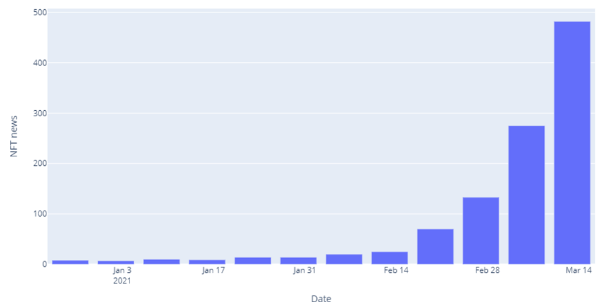
\includegraphics[width=12cm]{NFT-news-trends.png}
\caption{News trend in 2021 related to NFTs \autocite{dowling_fertile_2021}}
\end{figure}

The above figure shows the increase in news trends related to NFTs since the start of 2021. It has been exponentially increasing and hitting headlines around the globe on a daily basis.



% ----------------

\section{NFT Marketplaces}

% NFT Market places & what they offer. 

% Money in NFT & how markets have expanded (Open sea used by Reddit NFTs) and been funded.
OpenSea, which was the first NFT marketplace is also considered to be the largest. In the attempt to become the "Amazon of NFTs", OepnSea raised \$23 million in a Series A \autocite{hackett_this_2021}, following a \$100 million raise in a Series B round, ended the company in a valuation of \$1.5 billion \autocite{dfinzer_announcing_2021, matney_nft_2021}. Open Sea saw nearly \$150 million in sales in the month of June.

\begin{figure}[h!]
\centering
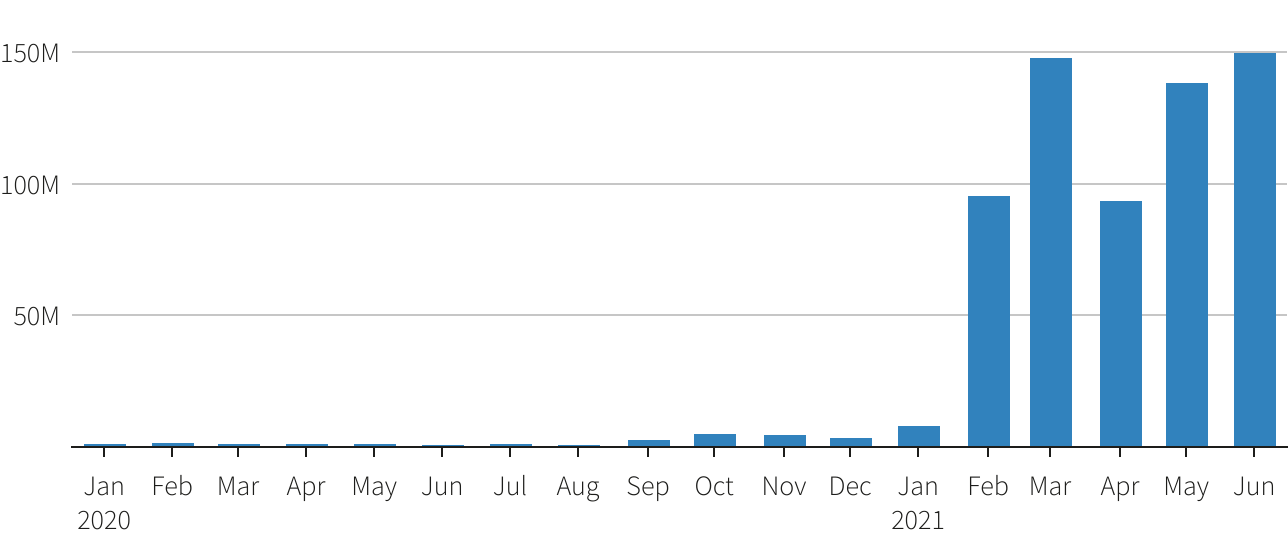
\includegraphics[width=12cm]{images/NFT-sales-opensea.png}
\caption{Monthly Ethereum-based NFT token sales volume on the OpenSea marketplace, in USD \autocite{howcroft_nft_2021}}
\end{figure}

% Mention other blockchains & marketplaces that sell NFTs
% Market places - OpenSea, Rarible, and Grimes’ choice, Nifty Gateway

These marketplaces are set to increase access to the digital goods industry.

An NFT purchased on an Ethereum marketplace can be traded on any other Ethereum marketplace for a completely different NFT. Creators don't necessarily need to sell their NFT on a market. They can do the transaction peer-to-peer, completely secured by Blockchain. No one is needed to intermediate and an owner isn't locked onto any platform \autocite{noauthor_erc-721_nodate}.

% How they can benefit from Recommendations - add to motivation? - already mentioned in problem



\section{Recommendation Systems}
Recommendation Systems have been driving engagement and consumption of content as well as items on almost every corner of the internet over the last decade.

\bigbreak

Recommendation Systems help users identify relevant items on an online platform. When users are recommended with relevant items, it enables businesses in growing their revenue. 35\% of Amazon’s revenue \autocite{naumov_deep_2019} \& 60\% of watch time on YouTube \autocite{noauthor_recommendations_nodate} comes from recommendations.


% ***\chapter{Problem Domain}
% Furthermore, they have to refer to several sources across the internet to find items that are highly trending.



% Although Computer Scientists and Data Scientists have pushed the limits of Recommendation Systems with recent advances in Machine Learning and Deep Learning, it is clear that none of the currently available Recommendation Architectures satisfies the thinking process identified by NFT owners & potential customers when searching for NFTs to trade.


\chapter{Problem Definition}
Currently, there is no way of identifying possible tradable NFT assets, unless manually browsing through the internet. 
Marketplaces allow searching for NFTs by keywords, categories \& pricing, but don't provide personalized recommendations of trending items.
This applies to someone who wants to purchase an NFT that shows similar characteristics to another NFT that has already been purchased by a previous buyer or oneself. Since there can be only one owner for an NFT at a time, recommendations using standard collaborative filtering is also not entirely ideal. Content-based approaches won't help identify trending items.

\bigbreak
In order to help with the exploration of these digital assets, it's identified that several steps that the user has to follow in order to identify trending items that are timely, popular among the community and may have an expected value can be automated. 

\section{Problem Statement}
It is difficult to find NFTs of comparable value that is trending among the community, timely and relevant to the user’s identified interest or the NFT that the user currently owns.

\chapter{Research Motivation}
% This has to be to the point!!!!
%  Refer to why it's important to solve this problem in NFTs
The problem identified in this proposal applies to both people who have a lot of domain knowledge about NFTs and people who have no idea how valuable items are in relation to their interests. Whoever it is, there's no solution that would mimic the exact thinking pattern of a person who is searching for a suitable NFT.

As mentioned in the work of \textcite{cheng_hybrid_2020}, Recommendation Systems play a significant role in the resolution of the problem of information overload. In order to provide ideal recommendations to a user, it is important to understand the user's thought process as well as other factors that affect a decision to trade.

% There have been many attempts to expand the capabilities of Recommendations by making use of public opinion. Collaborative Filtering was one approach to achieve that. Another identified approach was to make use of user-data on social media. This has been integrated into Machine Learning-based Hybrid Recommendation Architectures in many ways. In recent research done by Amazon \autocite{larry_history_2019} it is understood that when a timeline is considered for recommendations, an \emph{Autoencoder} Deep Learning model is capable of Recommending the best possible combination of movies to users.

Since the Recommendations domains are highly important for many business use-cases and the NFT domain is seeing a booming acceptance with a bright future ahead, this work is expected to add value to the progression of advancements \& accessibility related to the domains of NFTs, Blockchain \& Recommendation Systems.
% AI & Blockchain - extremely important technologies for businesses. This lets me get to work with both domains \autocite{} AI & Blockchain article
% *** mention that since NFTs are also originating from computer science, it's important to understand the factors that affect the pricing and market created by them - here?

\chapter{Existing Work}

\section{Recommendation Systems}
% \centering
\begin{longtable}{|p{0.17\linewidth}|p{0.07\linewidth}|p{0.15\linewidth}|p{0.23\linewidth}|p{0.23\linewidth}|} 
\hline
Research & Year & Technique Used & Improvements & Limitations \\ 
\hline
Amazon's Deep Learning-based movie recommendations model \autocite{larry_history_2019} & 2019 & Autoencoder, trained on chronologically sorted movie-viewing data & Outperformed item-to-item collaborative filtering  the bestseller list & \textit{Critique: The timeline doesn't consider overlapping of movies at various points in time, which will be necessary for trends.~}Tested only on movie recommendations. \\ 
\hline
A hybrid recommender system for the mining of consumer preferences from their reviews \autocite{cheng_hybrid_2020} & 2020 & A framework that integrates collaborative filtering with opinion mining  sentiment analysis on users' reviews that is used to create preference profiles. & Effective in dealing with insufficient data and is more accurate and efficient than existing traditional methods. The quality of recommendations can be improved regardless of whether the dataset is rich or sparse. & The semantic strategy of opinion extraction is generic. This may not be ideal to identify different aspects in varied genres. Slang, irony or sarcasm isn't considered in the current framework. It's very dependent on text mining of user reviews.~\textit{Critique: A person has to have placed reviews on previous movies in order to create a preference profile.} \\
\hline
User Rating Classification via Deep Belief Network Learning and Sentiment Analysis \autocite{chen_user_2019} & 2019 & A deep learning model to process user comments and to generate a possible user rating for user recommendations have been used. A Deep Belief Network and Sentiment Analysis (DBNSA) achieves data learning for the recommendations.~ & Outperforms baseline models in training loss value, precision, and recall on the Yelp and Amazon data sets. In the Trip-Advisor data set, DBNSA has the best MSE training loss value and recall.

DBNSA saves more time than the other baseline methods. & At present, the proposed method is not suitable for real-time testing. This method is required to be tested with a fast Deep Learning algorithm. Sarcastic comments have not been considered in user comments. \\ 
\hline
Cross-domain recommendations based on a hybrid approach \autocite{pes_universitydepartment_of_computer_science_bangalore_560085_india_cross-domain_2018} & 2018 & A hybrid approach of combination of content-based recommendation, user-to-user collaborative filtering and personalized recommendation techniques. & Address the limitations of single domain analysis such as data sparsity and cold start problem.

Integration of several domains is further capable of generating higher accuracy in suggestions.

Twitter sentiment analysis over the recommended entities generated by the model to help the user in decision making by knowing the positive, negative and neutral polarity percentage based on tweets done by people. & \textit{Critique: Sentiment analysis based on Twitter sentiment is calculated and shown after showing recommendations. It's ironic to recommend something and say if it's good/ bad by the system itself. Better if only positive sentiment-based items are recommended. }\\ 
\hline
 A LSTM-Method for Bitcoin Price Prediction\autocite{ferdiansyah_lstm-method_2019} & 2019 & LSTM (Long short-term memory). & The proposed model with time series techniques can predict the price for the next days with split the data to train and test. & The result is not good enough regarding the RMSE (Root Mean Squared Error). Future work: modified LSTM layers, adding dropout and modified number of epochs, and using different instability data-sets to test how good the prediction results are or~\textit{try to use sentiment analysis combined with LSTM method}~to see the impact of the uncertainty in value bitcoin. \\ 
\hline
Using basic machine learning to predict and recommend NFTs with OpenSea data  \parencite{noauthor_what_2020} & 2021 & Multiple Regression & This considers past purchase patterns, NFTs saved in wallets to predict if another wallet containing a similar combination will be likely to own an NFT from a specific category (eg: Cryptokitties, ENS domain, etc) in the future. & Recommends NFT categories that a user may be interested in. Doesn't recommend specific NFTs. The user needs to either manually input preferences or provide his wallet key that contains all his owned assets.~\textit{Critique: This won't consider current trends. It won't consider the recognition of the creators (eg: NFT made by Beeple).} \\
\hline
\caption{Related work in Recommendations Systems}
\end{longtable}


% Public Opinion - cheapest to get from social media & google trends

% ?***Crypto predictions using twitter data
% Abraham, J., Higdon, D., Nelson, J., Ibarra, J., 2018. Cryptocurrency Price Prediction Using Tweet Volumes and Sentiment Analysis 1, 22.
%? Netlify representation of recommendations


% Deep learning models - 
%X Facebook DLRM?, Embeddings Neu Embeddings?

%X Rendle, S., Krichene, W., Zhang, L., Anderson, J., 2020. Neural Collaborative Filtering vs. Matrix Factorization Revisited, in: Fourteenth ACM Conference on Recommender Systems, RecSys ’20. Association for Computing Machinery, New York, NY, USA, pp. 240–248. https://doi.org/10.1145/3383313.3412488


% ***this section might have to be changed?
\section{Understanding factors that affect NFT Markets}
% Facts to be considered related to NFTs when recommending
% \autocite{noauthor_off_2021} - price of NFTs have a relationship between the hype of the society and the interests of the community.
It is understood that the pricing of NFTs is moved by the changes in the pricing of cryptocurrencies, but appears to have comparatively less volatility. But the spillover between NFT markets has been identified to be very low compared to the high spillover effect among individual crypto markets \autocite{dowling_is_2021}.

The very first study done examining the pricing of NFTs suggests that \emph{"prospects for future studies are potentially limitless, as at the beginning of any new market"} \autocite{dowling_fertile_2021}. As a future study, the author has suggested identifying if there's a fundamental model that drives the price determination in NFTs.

% There're several factors that affect the desirablity of owning NFTs. When a person searches for NFTs he would be interested in knowing if the item is trending among the community - similar to the nature of crypto

% *** \/Related Work?
% CryptoKitties was one of the first NFT games & applications?
% Mention about NBA top-shot, Nike's CryptoKicks \autocite{}, artists work, etc. as industries that have stepped into the NFT craze and then...
% how the technology will evolve in the future.

% *** figure \autocite{noauthor_erc-721_nodate} - The comparison between NFT internet & the internet today can be used to show the value of NFTs in the thesis.


\emph{"The value of an NFT is entirely determined by what someone else is willing to pay for it."} \autocite{conti_what_2021}
% "As a result, demand will drive the price rather than fundamental, technical, or economic indicators, which typically influence stock prices and, at the very least, serve as the basis for investor demand".

\emph{"Ultimately owning the real thing is as valuable as the market makes it. The more a piece of content is screen-grabbed, shared, and generally used the more value it gains. Owning the verifiable real thing will always have more value than not."} \autocite{noauthor_erc-721_nodate}

These statements prove that the demand for investment in NFTs will be heavily reliant on the public's acceptance of the item is.

% ----------------


% \begingroup
% \let\clearpage\relax 
% summarize & point out why research is required
% Considering the above-mentioned points, 
\chapter{Research Gap}
Based on previous work done related to Recommendation Systems, the literature doesn't identify integrating all the factors that affect the desirability of owning relevant, timely \& trending NFTs (items) to a recommendations model. This project focuses on an Empirical gap in the NFT domain as well as Theoretical and Performance gaps in Recommendations Systems. 
% Empirical gap - research that is based on observation and measurement of phenomena, as directly experienced by the researcher. 

Collaborative filtering, which has been a standard baseline technique for Recommendations for over a decade, can't be taken as the only recommendations model because, by the time one NFT is viewed many times by other users, it may already be too late for another user to purchase that item.


\chapter{Research Contribution}

% *** this will come to a solution? The main challenge when it comes to recommending NFTs to users is that the Recommendations System has to know what items are trending in the world while being relevant.

% \bigbreak
The author's research contribution can be summarized as follows:
\begin{itemize}
\item \textbf{Recommendations Systems}: Data Engineering + Data Science [\Gls{ml} + \Gls{dl}] + Ensemble models
\item \textbf{NFT Trading}: Recommendations + \Gls{ai} + Automation + Data Analysis
\end{itemize}

\section{Technological Contribution}

A Hybrid Recommendations technique that attempts to use public trends in a way that hasn't been attempted in previous research will be explored in order to facilitate the recommendation of relevant, trending and timely items. Automation of several decision-making steps that a user would otherwise need to go through to find the best possible trade will be integrated into the Recommendations Architecture. It is hypothesized that this novel recommendations architecture will be able to be applied to other items as well in order to give enhanced recommendations based on trends.

\section{Domain Contribution}

The information in an NFT that has an effect on a user's desire to be owned will be identified, when attempting to provide suitable recommendations.
Looking at the success of Recommendation Systems across multiple systems for over a decade, it is understood that a Recommendation System would help users identify NFTs that they would be interested in trading. This will in return help in increasing sales on NFT Marketplaces and wider adoption of the technology.

\bigbreak
NFTs are a result of the advancement of the application of techniques related to Blockchain, while Recommendation Systems are a result of Data Science advancements over the last few decades. Both the domains considered in this research can be identified to be originated from the field of Computer Science.


\chapter{Research Challenge}
NFTs is a new domain, which has very less research done related to preferences and factors considered when purchasing NFTs.
Therefore, it is first important to identify the data points (features) \& external factors that affect the value/ desirability of owning NFTs to suggest trading recommendations of NFTs to a user.

\bigbreak
% add this to challenge?
\textit{"Crypto has a founding tradition of emphasizing freedom and privacy. Maybe because of this prevailing cultural trend, the NFT space does not have many recommender systems."} \autocite{noauthor_what_2020}

NFTs are identified to be more challenging to be recommended to users using traditional recommendation methods due to the uniqueness of each item together with the traditions brought forward with the crypto community.
Similar to cryptocurrencies, it has been identified that NFTs too have an impact on the general public opinion \& trends \autocite{dowling_fertile_2021}.

Currently, available Recommendation Systems haven't had the necessity to consider trends as much as with related to the desirability of owning NFTs. Furthermore, scarcity of items opens another challenge of the inability to keep recommending items that are not available for sale or have already been purchased by an interested buyer. But that alone can't be considered due to the time-tested \& proven baseline recommendation techniques being highly effective in multiple domains. Using the identified factors to be considered, a suitable recommendations architecture needs to be implemented.

\chapter{Research Questions}

\begin{itemize}[label={}]
  \item {\textbf RQ1:} What are the features of NFTs \& external factors that affect the desirability of owning NFTs?
  \item {\textbf RQ2:} How can a system predict the most relevant, trending, timely \& worthy NFTs for trading purposes?
  \item {\textbf RQ3:} What are the recent advancement in recommendation models \& architectures that can be taken into consideration when building a hybrid Recommendation Architecture, using ensemble techniques? 
\end{itemize}

\chapter{Research Aim}
\textit{The aim of this research is to design, develop \& evaluate a novel Recommendation Architecture that will provide relevant, trending, timely, and worthy NFTs for trading purposes by automating some of the decision making steps that the user would otherwise have to do manually.}

\bigbreak
To elaborate on the aim, this research project will produce a system \& architecture that can be used to recommend trending items with respect to a chosen item in a specific data set. The focus will be laid on the recommendation of NFTs. In order to achieve this several public channels of trends will be required to be streamed into the recommendations architecture together with the automation of several decision-making steps that a user that is interested in purchasing NFTs would have to manually go through, in order to make the best possible trade. The use of Data Mining techniques, \Gls{nlp} techniques, Data Analysis, hybrid, content-based, collaborative filtering \& Deep Learning methods will be researched to make the best possible recommendations.

The required knowledge will be studied and researched, components will be developed and the performance will be evaluated in order to validate or invalidate the chosen hypothesis. The system will be able to run in a local browser for personal use or in a hosted server for public use. The data science models \& their code will be available for further research and use in a public repository that is easy to get up and running with ease. A review paper will be published with knowledge gathered from the survey of Literature. A research paper will be published on the outcome of the findings in the research project.

\chapter{Research Objectives}
The Aims and Research Questions mentioned above are expected to be achieved and answered with the completion of the following Research Objectives. These objectives are milestones that will be expected to be met in order for the research to be completed successfully.

%  ***breakdown all the rows into atomic objectives to be done

% \begin{table}[h!]
% \centering
\begin{longtable}{| p{0.23\linewidth} | p{0.58\linewidth}| p{0.12\linewidth}|}
\hline
Objective &   Description & Learning Outcomes  \\ 
\hline
Problem Identification & Identifying a suitable and valuable problem domain to contribute towards, with identified research gaps suitable for a research project & LO5 \\
\hline
Literature Review & Read previous work to collate relevant information on related work and critically evaluate them & LO4, LO2, LO5 \\
\hline
Project Methodology & Choosing the Research, Development and Project Methodologies that can be followed. Creating a project plan with expected activities and scheduled times for the time-frame allocated for the project & LO3, LO7 \\
\hline
Requirement Specification & Specifying the requirements of the project using appropriate techniques and tools in order to meet with the expected research gaps \& challenges to be addressed & LO1, LO2, LO5, LO7\\
\hline
Data Gathering and Analysis & Collecting and analysing data used in previous related research and any domain-specific data required to solve the research problem  & LO1, LO5 \\
\hline
Research Design & Designing architecture and a system that is capable of solving the identified problems with recommended techniques. & LO1 \\
\hline
Implementation & Implementing a system that is capable of addressing the gaps that were aimed to be solved. & LO1, LO5, LO6 \\
\hline
Testing and Evaluation & Testing the created system \& Data science models with appropriate data and evaluating them with baseline techniques identified in literature & LO4 \\
\hline
Documenting the progress of the research & Documenting and notifying the continuous progress of the research project and any faced obstacles. & LO8, LO6 \\
\hline
Publish Findings & Producing well-structured documentation/ reports/ papers that critically evaluate the research.
\begin{itemize}
\item Publishing a review paper on related work.
\item Publishing evaluation \& testing results identified from the research.
\item Making the code or models created in the research process available for future advancements in research.
\item Making any modified data-sets or re-creation strategies available to the public, to train \& test models related to similar use cases of utilized data.
\end{itemize}
& LO4, LO8 \\
\hline
\caption{Research Objectives}
\label{tab:research-objectives-table}
\end{longtable}
% \end{table}


\chapter{Project Scope}
The scope is defined as follows based on the project objectives and a review of existing products with consideration to the granted time period for this research project.

\section{In-scope}
The following is a list of the project's scope:
\begin{itemize}
\item A system that is capable of recommending NFTs to users based on a specific NFT chosen by a user.
\item Creation of a Recommendations System that integrates public trends on social media.
\item Creation of a Recommendations System that is capable of providing better rending recommendations compared to baseline techniques.
\item Testing the requirement of integrating public trends into a Recommendations architecture with the use of Content-based filtering, collaborative filtering \& Deep Learning techniques.
\item \Gls{gui} that allows a user to provide the tokenId of a chosen NFT by the user \& to view the results given by the Recommendations System.
\item Automation techniques with related to Smart Contracts will be directly applicable only to selected Blockchains.
\end{itemize}

\section{Out-scope}
The following are the parts that will not be covered by the project:
\begin{itemize}
\item Recommending items that haven't been seen previously by the system.
\item Creating a Recommendations System that utilizes less computational power \& resources compared to baseline techniques.
\item GUI with options to tune the Recommendations System.
\item All automation techniques to cover every available Blockchain.
\end{itemize}

\section{Prototype High-Level Architecture Diagram}
% a diagram is needed here - use Figma diagram?
% ***


% ***Processing an initial review of literature, _ key components were identified to create a Recommendation System suitable for NFT Trading recommendations.
% (Data Collection - NFTs, Opinion Mining, NLP matching stage, Content-based filtering + collaborative filtering => Deep Learning model - Autoencoder)
% 1.

\chapter{Proposed Methodology}

\section{Research Methodology}
The quality of any project is governed by three key factors: cost, time, and scope, all of which must be managed efficiently throughout the project's lifetime. As a result, methodologies are required. Saunders  Research Onion Model \autocite{writers_saunders_2019} has been used to deduce the methodologies. 
The methodologies chosen as appropriate for the project are listed in the table below.

\begin{longtable}{| p{0.22\linewidth} | p{0.75\linewidth}|}
\hline
Research Philosophy  & The philosophy of research influences data collection \& data analysis since it is related to the nature of reality being investigated.

Positivism, Interpretivism \& Constructivism are philosophies that could be used to approach this research. Out of these, \textbf{Positivism} was chosen since the research is expected to be replicable with similar \textbf{quantifiable} results.
\\
\hline
Research Approach & The approach that a researcher may use when conducting the research is the approach.

A \textbf{Deductive} approach was chosen over an Inductive approach since this is expected to be a \textbf{quantitative} research that aims to \textbf{test \& prove} the \textbf{hypothesis} at hand. \\
\hline
Research Strategy  &The strategy focuses on the data collection methods that will be used to answer the research questions.

\textbf{Survey, Archival Research} \& \textbf{Ethnography} were the strategies chosen to address the research questions. These strategies were chosen as they would compliment each other while providing relevant data that is enough for the research. While Survey seems to be the primary strategy, Archival Research \& Ethnography is expected to allow the \textbf{qualitative aspect} expected in the approach taken to the solution, which will finally affect the \textbf{quantitative results}, to be addressed. \\
\hline
Research Choice & Choice of the methodology identifies if the research is concerned with the qualitative and quantitative aspects of the research.


\textbf{Multi-method} was chosen since although \textbf{quantitative results} are the primary  perspective, it is identified that \textbf{qualitativeness} of the data used by the system to be developed will also be an important consideration that will affect the quantitative results.\\
\hline
Time Horizons  & 

\textbf{Longitudinal} was chosen as the time horizon for the research since data will be gathered and used for evaluation and testing over a long period of time.\\
\hline
Techniques and procedures &  Data collection and analysis techniques are considered here.

Mediums such as online news, statistics \& trends from social media, observations, conversations, reports, surveys, documents, secondary tabular data, organizational records will be used.\\
\hline
\caption{Research Methodology}
\label{tab:research-methodology-table}
\end{longtable}


\section{Development Methodology}
\subsection{Life cycle model}
\textbf{Agile} Software Development Life-cycle was chosen as the research development method since iterative development is needed. \textbf{Prince2}  was chosen as the product development methodology. It allows the author to develop the product in controlled environments in logical compartmentalized units.


\subsection{Design Methodology}
% SSADM or OOAD or Anything else?
Object-Oriented Analysis and Design were chosen as the Design Methodology by the author to support an incremental methodology that can be used to extend the system with the ability to reuse system components.

\subsection{Evaluation Methodology}
As identified in recent advancements in literature \autocite{larry_history_2019}, \gls{p@k} score has been identified as a suitable method of bench-marking a recommendations system for evaluation purposes. Therefore, it will be used to compare the novel solution that is to be developed against baseline models.

\section{Project Management Methodology}
\newpage
\subsection{Scheduled Timeline}
% Gantt Chart
\begin{figure}[h!]
\centering
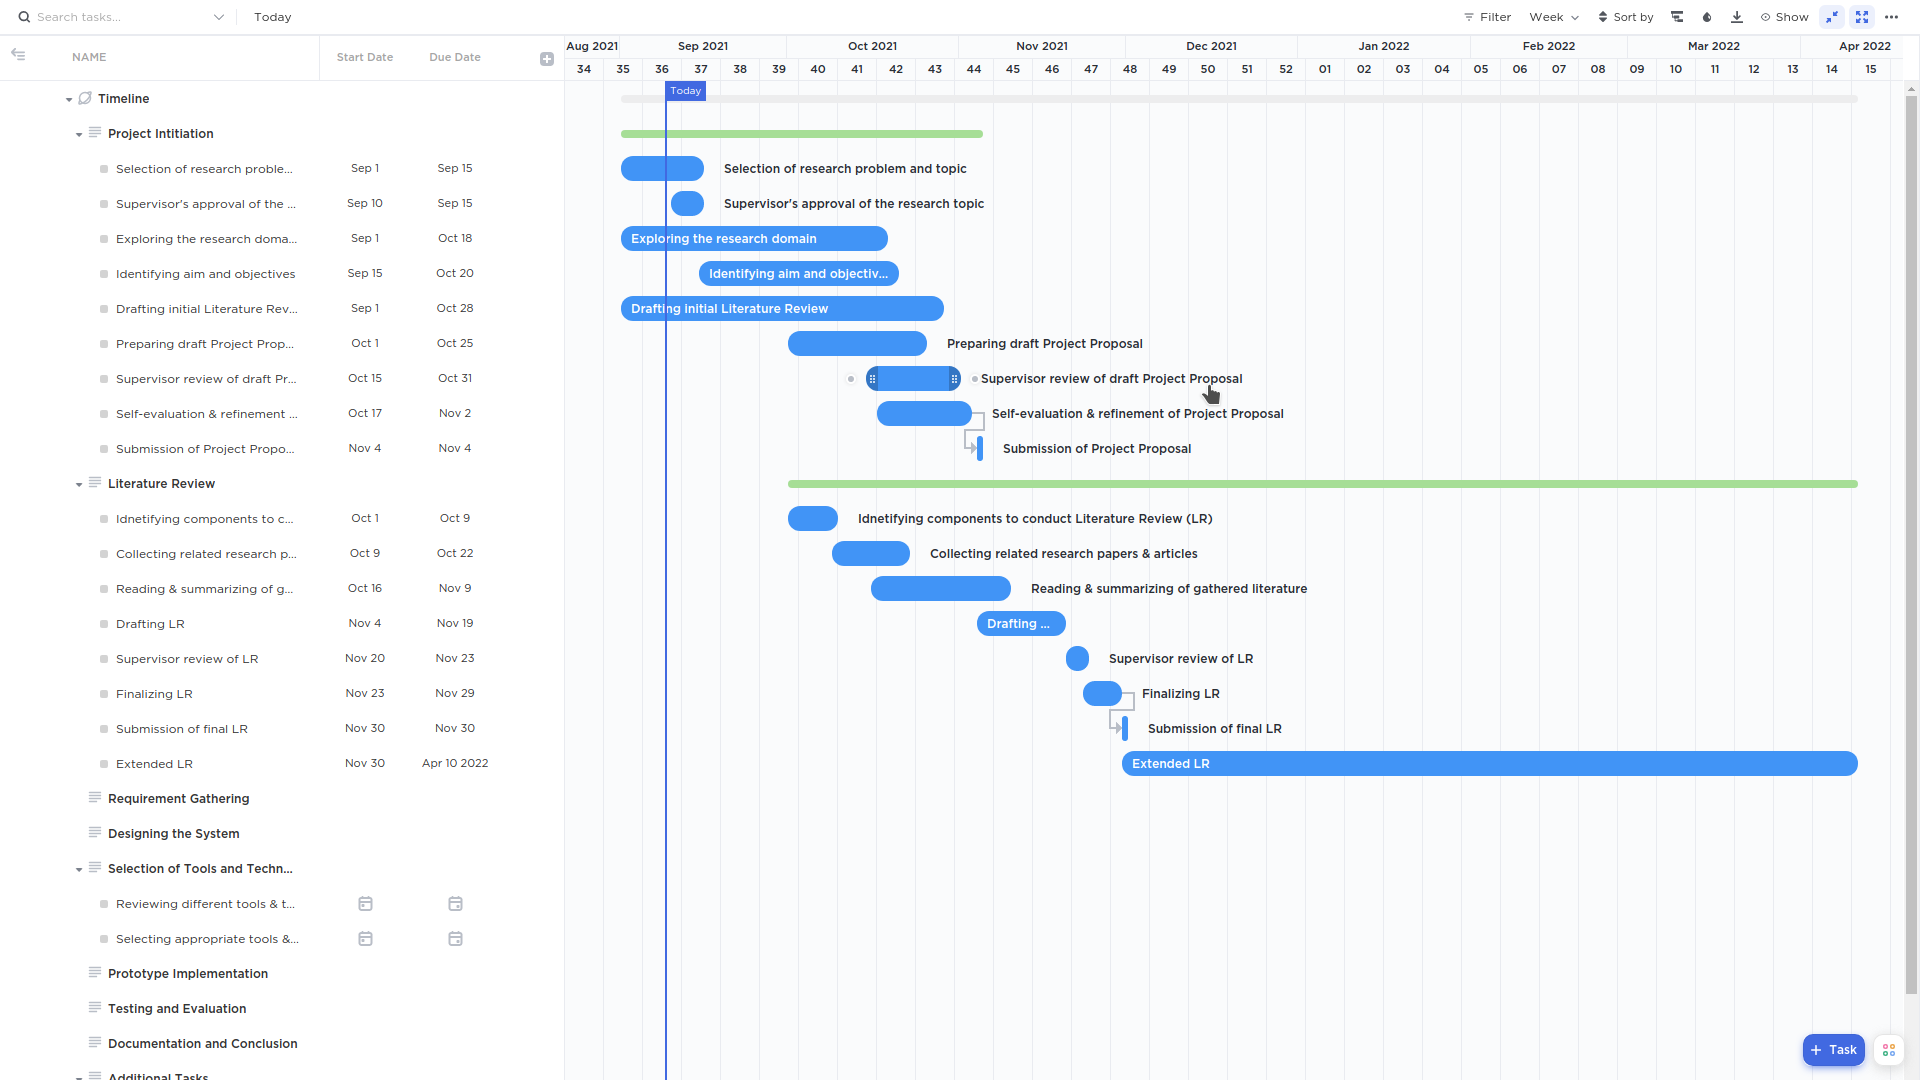
\includegraphics[width=\textwidth]{images/gantt-chart.png}
\caption{Gantt Chart}
\end{figure}


\newpage
\subsection{Deliverables}

% \centering
\begin{longtable}{| p{0.76\linewidth} | p{0.22\linewidth}|}
\hline
Deliverable &   Date  \\ 
\hline
\textbf{Project Proposal Document}    &   4\textsuperscript{th} November 2021\\
% \cline{1-1}
The initial proposal of the project  &  \\ 
\hline
\textbf{Literature Review Document} & 11\textsuperscript{th}~December 2021  \\ 
The Critical review of existing work and solutions  & \\ 
\hline
\textbf{Software Requirement Specification} & 15\textsuperscript{th}~December 2021 \\ 
The document specifying requirements to be satisfied and developed as the final prototype and means of collecting data &    \\ 
\hline
\textbf{System Design Document} & 1\textsuperscript{st}~December 2021  \\ 
The document specifying the design developed for the Recommendations System and overviews of the algorithms to be developed.    &   \\ 
\hline
\textbf{Prototype}  & 1\textsuperscript{st}~February 2022   \\
The prototype with main core features functional    &    \\ \hline
\textbf{Thesis} & 15\textsuperscript{th}~March 2022  \\  The final report documenting the project and research process and decisions          &   \\ 
\hline
\textbf{Review Paper}  &  1\textsuperscript{st}~March 2022     \\ 
A review paper reviewing existing systems in the Recommendations domain published in a journal/ conference    &   \\ 
\hline
\textbf{Manuscript Paper}   &  31\textsuperscript{st}~December 2021 \\ 
A research paper introducing the concepts and design developed as part of this project &   \\ 
\hline
\textbf{Final Research Paper}   &   1\textsuperscript{st}~April 2021    \\ 
A research paper introducing the Recommendations System developed at the end of this project    &    \\ 
\hline
\textbf{Public project library}   &   1\textsuperscript{st}~April 2021 \\ 
A publicly accessible project library/ repository to set up, test and use the developed Recommendations System  &   \\
\hline
\caption{Deliverables and dates}
\label{tab:deliverables-table}
\end{longtable}

\subsection{Resource Requirements}
The resources required to complete the project are identified based on the objectives, expected solutions, and deliverables. The following are the software, hardware, and data resource requirements.

\subsubsection{Software Requirements}
\begin{itemize}
\item \textbf{Operating System(Linux/ macOS/ Windows 10)} - Linux will be the default choice for development since of the ease of support for multiple development tools and performance benefits. macOS/ Windows will be used for research documentation \& study purposes.
\item \textbf{Python} - The language that will be used to create the Machine Learning \& Deep Learning models. Python is an all-purpose language that has been used in many projects that integrate with data science.
\item \textbf{Tensorflow/ Scikit learn Python packages} - Libraries that will be used to support model development, training \& testing.
\item \textbf{Golang/ NodeJS} - The Application Programming interface that will be used to communicate with the \Gls{ml} backend and the front-end. Golang will allow the application to support concurrency and multi-threaded communications while being extremely lightweight and fast. This will be used to avoid any bottlenecks that could occur at this point in the system. NodeJS will be kept as a secondary option in the case of requiring any pre-built features that are not directly supported by Golang \& aren't directly relevant to the research.
\item \textbf{JavaScript (React)} - The front-end of the application, where recommendations will be shown. This is also an important part of the project since it will be the users' point of interaction with the system.
\item \textbf{PyCharm/ VSCode/ GoLand} - Development environments to support development of the project.
\item \textbf{Google Colab} - Cloud development environment to build, train \& test ML \& Deep Learning models.
\item \textbf{Zotero} - Research management tool to save and backup research artifacts \& manage references.
\item \textbf{Overleaf/ MS Office/ Google Docs/ Canva/ Figma} - Tools to create reports, figures \& documentations.
\item \textbf{Google Drive/ GitHub} - To backup files \& code related to the project
\item \textbf{Docker} - To make the ensemble system's setup process as simple as possible.
\end{itemize}

\subsubsection{Hardware Requirements}
\begin{itemize}
\item \textbf{Core i7x Processor(8\textsuperscript{th} generation)} - To be able to perform high resource intensive tasks.
\item \textbf{Nvidia 1050Ti GPU} - To manage training processes of data science models.
\item \textbf{16GB RAM} - To manage data-sets \& development environments.
\item \textbf{Disk space of 40GB or above} - To store data \& application code.
\end{itemize}

\subsubsection{Data Requirements}
\begin{itemize}
\item \textbf{Non-fungible Token data} - From OpenSea open-API.
\item \textbf{Twitter data} - From Twitter developer API.
\item \textbf{Google Trends data} - From Google Dataset Search \& unofficial Google Trends Python API (Pytrends).
\item \textbf{Ethereum Smart Contract data} - From Etherscan
\item \textbf{User Preference Profiles data} - From Amazon, Yelp, Kaggle open datasets. May be needed for testing purposes.
\end{itemize}

\subsubsection{Skill Requirements}
\begin{itemize}
\item Creation of required Recommendation Systems.
\item Ability to create optimized Machine Learning \& Deep Learning models.
\item Research writing skills.
\end{itemize}

\subsection{Risk Management}
The following are the risks identified prior to starting the project with possible mitigation steps.
\begin{longtable}{| p{0.33\linewidth} |p{0.11\linewidth}| p{0.11\linewidth}| p{0.34\linewidth}|}
\hline
Risk Item & Severity & Frequency & Mitigation Plan \\
\hline
Loose access to on going development code & 5 & 2 & Keep all code backed up on GitHub \& external backup \\
\hline
Corruption of documentation & 4 & 4 & Follow a cloud-first documentation approach and backup on a weekly basis \\
\hline
Inability to complete all expected deliverables within the allocated time & 4 & 2 & Work on deliverables on a priority basis. \\
\hline
Inability to explain the research work done due to illness & 2 & 1 & Have a recording of demonstration and detailed documentation with explanation \\
\hline
\caption{Risk Mitigation Plan}
\label{tab:risk-mitigation-table}
\end{longtable}

\endgroup

% *** Appendix: Concept Map

\newpage
% BIBLIOGRAPHY-----------------------------------------------
\printbibliography[heading=bibintoc, title = {References}]


% *** add concept map to appendix?

\end{document}